\documentclass[11pt,a4paper]{article}
\usepackage[margin=2.6cm]{geometry}
\usepackage[T1]{fontenc}
\usepackage[utf8]{inputenc}
\usepackage{amsmath}
\usepackage{booktabs}
\usepackage{graphicx}
\usepackage[hidelinks]{hyperref}
\usepackage{natbib}
\usepackage{setspace}
\usepackage{tabularx}
\usepackage{pdflscape}
\usepackage{tikz}
\usetikzlibrary{positioning,arrows.meta}
\onehalfspacing

\title{From Supply and Use Tables to Reproducible Social Accounting
Matrices:\\ A Transparent Construction and Audit Framework\\
\large Evidence from three publication regimes: South Africa, Kenya,
and the Netherlands --- working paper, draft v0.8}
\author{Kodzovi Abalo\thanks{World Bank. The views expressed here are those
of the author and do not necessarily reflect the views of the World Bank,
its Executive Directors, or the governments they represent. Comments
welcome.}}
\date{July 2026}

\begin{document}
\maketitle

\begin{abstract}
\noindent
Social accounting matrices (SAMs) underpin much applied policy modelling,
yet the way they are built has a reproducibility problem: heterogeneous
official tables are reconciled through undocumented spreadsheet operations
and expert judgments that cannot be audited, updated, or transferred. This
paper demonstrates that the problem is unnecessary---that SAM construction
can move from an artisanal exercise to an auditable statistical-production
process. We introduce a construction and audit framework in which every
source is fingerprinted, every classification and formula is
machine-readable, every balancing adjustment is logged at the cell where
it acts, and accounting identities are enforced as executable checks. We
apply it to build a complete 2019 SAM for South Africa from publicly
obtainable official sources and access-controlled survey microdata,
audited cell by cell against the published UNU-WIDER benchmark of
\citet{vanseventer2023}: the benchmark's production and commodity
structure is reproduced exactly, and its institutional macro structure is
reproduced exactly except for one unpublished input---separately
identified and priced ($+16.1$ per cent on import duties under its public
proxy)---and one bounded unrecorded reconciling adjustment. Where the benchmark's choices are
undocumented, the framework recovers them numerically; every reported
discrepancy was first detected by deterministic reconciliation and then
interpreted against the source record. Two further, deliberately
shallower applications test the framework at the ends of the public-data
spectrum: in Kenya, auditing proceeds exactly as far as the boundary set
by publication format; in the Netherlands, the framework generates and
balances a macro SAM from three Eurostat API calls with no benchmark
consulted. The open toolkit that implements the framework is offered as
reproducible infrastructure, and the central proposal follows: cell-level
provenance and machine-readable construction rules, published alongside
every SAM, would make such audits---and such SAMs---routine.
\end{abstract}

\vspace{0.5em}
\noindent\textbf{Keywords:} social accounting matrix, supply and use tables,
reproducibility, data provenance, statistical auditing, South Africa,
Kenya, Netherlands.\\
\textbf{JEL:} C67, C82, D57, E16, O55.

\section{Introduction}\label{sec:intro}

Social accounting matrices organise an economy's transactions---production,
factor incomes, institutional transfers, accumulation, and external
flows---into a single square array in which every account's receipts equal
its payments. They are the standard database for multiplier analysis and
computable general equilibrium modelling, and in many countries they are the
principal quantitative bridge between official statistics and policy
simulation.

Yet SAM construction has a reproducibility problem. The way matrices are
built has changed remarkably little since \citet{pyattround1985}:
heterogeneous official tables are reconciled through long chains of
spreadsheet operations, expert judgments, and balancing passes that are
rarely documented at the level where they act---the individual cell. The
consequences are familiar to every practitioner: published SAMs are trusted
and used, but they can seldom be reproduced, audited, or updated by anyone
other than their authors; knowledge of how a matrix was actually built
leaves when its builder does; and each new country or benchmark year
restarts the work nearly from scratch. Section~\ref{sec:related} argues
that this is a property of the prevailing \emph{medium}---prose describing
spreadsheets---rather than of any particular team.

This paper demonstrates that the problem is unnecessary: SAM construction
can move from an opaque artisanal exercise to an auditable, executable
statistical-production process. We introduce a construction and audit
framework with four commitments: every source file is fingerprinted and
registered; every classification, concordance, and cell formula is
machine-readable and reviewable; every balancing adjustment is logged at
the cell where it acts; and the accounting identities that define a SAM
are enforced as executable checks rather than assumed. We then apply the
framework end to end, building a complete 2019 SAM for South Africa from
publicly obtainable official sources and access-controlled survey
microdata---inputs available to any researcher at no cost, with no
privileged access\footnote{``Publicly obtainable'' means: published
statistical releases plus survey microdata obtainable by any registered
researcher under DataFirst's standard access conditions. The one input
that is not obtainable at all---the benchmark's unpublished customs
figure---is treated separately and priced
(Section~\ref{sec:results:macro}); the \emph{public-proxy} scenario of
our SAM uses published sources only.}---and auditing it, cell by cell,
against the strongest available benchmark: the 2019 South African SAM
published by UNU-WIDER \citep{vanseventer2023}, which is unusually well
documented by the standards of the genre and ships with a technical note
mapping its macro structure to South African Reserve Bank (SARB)
national-accounts series.

South Africa is the evidence, not the point. The audit produces three kinds
of result that we argue generalise. First, \emph{exact replication where
the sources allow it}: the benchmark's entire production and commodity
side reproduces from the official supply and use tables to within
R0.5~million on all 61 activities and all commodities, and 43 of 45
computable institutional macro cells match the SARB series exactly
(Table~\ref{tab:headline} summarises). Second, \emph{numerical recovery of
undocumented choices}: where the benchmark's documentation is silent or
mistaken, the data identify what was actually done---the edition and
measure behind its capital-stock split, the unique sign structure of a
misprinted aggregation formula, and the household grouping variable.
Third, \emph{a priced replicability boundary}: the benchmark rests on
exactly one non-public input, and substituting its public proxy changes
import duties by $+16.1$ per cent and product taxes by $-1.5$ per cent; a
small unrecorded balancing adjustment and a handful of sector-level share
edits are likewise isolated and measured---each detected because it left
an arithmetic trace, which is the limit of what this method can claim.

Two further applications then place South Africa on a spectrum, and the
three-country design is deliberately asymmetric: one deep audit, one
data-boundary test, one transfer-and-generation demonstration. The
applications are not three comparable country studies---each answers a
different question about the same framework under a different publication
regime, and their unequal depth is the research design, not uneven
execution. Applied to Kenya---where the machine-readable supply--use
detail behind IFPRI's widely used 2019 SAM is not published---the
framework verifies the matrix's structure and macro controls against the
national accounts and locates exactly where verification must stop: the
published accounts carry a statistical discrepancy of 3.6~per~cent of
GDP, a balanced SAM cannot carry one, and the deviation pattern is
consistent with the discrepancy being absorbed primarily through the
consumption and trade aggregates. Applied to the Netherlands---where
harmonised tables are a public API---the framework needs no benchmark at
all: three API calls, a 70-line reader, and one script generate a 2019
macro accounting matrix whose inputs pass every identity exactly and
whose residuals are each attributed to a named ESA boundary item, and a
logged balancing step then closes it into a macro SAM
(Section~\ref{sec:applications}).

Our contribution is therefore not a new balancing estimator. That
literature is active rather than closed---cross-entropy estimation
\citep{robinson2001}, GRAS for matrices with negative entries
\citep{junius2003,temurshoev2013}, and KRAS for conflicting and
unequally reliable constraints \citep{lenzen2009} each address a
different compilation problem---and this paper adds nothing to it. What
we contribute instead is a demonstration, on a full-scale
national SAM, of five things at once: a reproducible construction pipeline;
an audit methodology whose discrepancies are detected by
\emph{deterministic reconciliation against accounting identities} rather
than by reading documentation; a reconstruction of a published national SAM
from publicly obtainable sources with every departure disclosed and
quantified; a
taxonomy of the ways documentation and data diverge in even the
best-documented matrices; and an open toolkit---readers for supply--use,
SAM, central-bank, and survey sources; concordance and account-taxonomy
machinery; RAS balancing with mandatory diagnostics; a generator for
workbooks whose totals and balance checks are live formulas---offered as
reproducible infrastructure for official SAM construction and released
with the replication package.\footnote{The toolkit (\texttt{edikit}) and
all scripts, registries, and derived tables are part of the replication
package; see the Reproducibility and AI disclosure section.} The framework
doubles as a practical construction workflow: the pipeline generates and
balances the matrix mechanically, so that scarce expert time is spent only
on the residual cells that identities cannot determine
(Section~\ref{sec:discussion:workflow}).

The idea the paper keeps returning to is simple: \emph{cell-level
provenance and machine-readable construction rules, published alongside
every SAM, would make such audits---and such SAMs---routine.} The paper
proceeds as follows. Section~\ref{sec:related} situates the work and
contrasts the prevailing construction workflow with the framework's.
Section~\ref{sec:data} describes the source registry.
Section~\ref{sec:method} sets out the pipeline and the audit method.
Section~\ref{sec:results} reports the South African replication block by
block. Section~\ref{sec:applications} presents the Kenyan and Dutch
applications and the replicability spectrum they trace.
Section~\ref{sec:discussion} draws out the taxonomy, the construction
workflow, and implications for statistical practice, and
Section~\ref{sec:conclusion} concludes.

\section{Background: the practice and its reproducibility problem}
\label{sec:related}

\subsection{Related work}

The SAM as an integrated accounting framework descends from
\citet{stone1962} and was consolidated as a planning tool by
\citet{pyattthorbecke1976} and \citet{pyattround1985}. The mechanics of
reconciling inconsistent accounts are equally mature: biproportional (RAS)
adjustment and its generalisations \citep{temurshoev2013}, and the
cross-entropy estimation of \citet{robinson2001}, which remains the
standard reference for SAM balancing under scattered and unequally reliable
information. Compilation practice for the supply--use core is codified in
the SNA and its handbooks \citep{un2009sna,un2018handbook,eurostat2008};
the analytics that consume SAMs are surveyed by \citet{millerblair2009}
and, for CGE databases, \citet{lofgren2002}. Operationally, most African
country SAMs are produced within a small number of institutional
pipelines---notably IFPRI's country programmes \citep{thurlow2021} and
UNU-WIDER's South Africa series---of which the benchmark used here
\citep{vanseventer2023} is a leading example.

The paper's infrastructure claims sit at the junction of several
adjacent literatures, each of which has solved a piece of the problem.
Large international input--output databases are compiled under documented,
code-driven procedures---WIOD \citep{timmer2015}, EXIOBASE
\citep{stadler2018}, and Eurostat's FIGARO tables \citep{remond2019}---and
open-source tooling such as \texttt{pymrio} \citep{stadler2021} has made
their \emph{consumption} programmatic; but these systems document
methodology at the level of reports, not cell-level provenance, and none
is designed to let an outsider audit a single published matrix against
its own record. Machine-readable statistical standards (SDMX for
dissemination \citep{sdmx2021}; the W3C PROV model for data lineage
\citep{w3cprov2013}) supply exactly the vocabulary our standards proposal
needs, but have not been applied to SAM construction. And the norms of
reproducible computational research---\citet{peng2011},
\citet{sandve2013}, and for economics practice
\citet{gentzkow2014}---prescribe the workflow discipline the framework
implements, without the accounting-identity instrument that makes SAM
auditing unusually sharp. Within economics the paper joins the
transparency and replication agenda \citep{christensen2018}, with that
accounting twist: a SAM's identities give the auditor a powerful
instrument, because any undocumented intervention must either break an
identity or leave a biproportional fingerprint. To our knowledge, no
existing system combines registered sources, executable identities,
cell-level provenance, and logged balancing for national SAM
construction---which is why, as Section~\ref{sec:related:workflow}
argues, a full cell-level replication audit of a published national SAM
appears not to have been undertaken before.

\subsection{Why current workflows resist reproduction}
\label{sec:related:workflow}

The prevailing construction workflow---official tables copied into
spreadsheets, reconciled by hand, described afterwards in prose---fails
five requirements at once, none of them because practitioners are careless
(Table~\ref{tab:workflow}). \emph{Transparency}: judgments act on
individual cells but are reported, if at all, at the level of methods
paragraphs. \emph{Versioning}: a spreadsheet's history is its author's
memory; source vintages and revisions are rarely pinned.
\emph{Provenance}: a finished cell does not say which source, which
transformation, and which manual edit produced it. \emph{Auditability}: a
reader can check that the matrix balances, but not why any cell holds its
value. \emph{Reproducibility}: rebuilding the matrix from its stated
sources is a research project, not a command---as this paper demonstrates
by undertaking exactly that project. To our knowledge it is the first
full cell-level replication audit of a published national SAM from primary
sources; that such an audit is novel is itself evidence of the problem.

\begin{table}[t]
\centering\small
\caption{Prevailing SAM construction workflow versus the framework used here.}
\label{tab:workflow}
\begin{tabularx}{\textwidth}{lXX}
\toprule
Requirement & Prevailing practice & This framework \\
\midrule
Transparency & Judgments described in prose, if at all & Classifications, formulas, and rules are machine-readable files \\
Versioning & Source vintages implicit; spreadsheet history unrecorded & Every input registered with vintage, access date, SHA-256 hash \\
Provenance & Finished cells carry no origin & Cells trace to source series, transformation, and logged adjustment \\
Auditability & Balance checkable; cell values not & Identities enforced as executable checks; adjustment log published \\
Reproducibility & Rebuild is a research project & Rebuild is a command (scripts 01--12 of the replication package) \\
\bottomrule
\end{tabularx}
\end{table}

\section{Data}\label{sec:data}

Every input is recorded in a source registry with publisher, vintage, access
date, licence status, and SHA-256 hash; raw files are never modified, and
artefacts derived from them carry lineage to the registry entry. The South
African sources are:

\begin{itemize}
  \item \textbf{Supply and use tables} (Stats~SA Report 04-04-03): the
  2018--2019 workbook with supply and use tables at 124 industries and 108
  products, plus the accompanying methodological report. These are the sole
  inputs to the production and commodity blocks.
  \item \textbf{Benchmark SAM} (UNU-WIDER Technical Note 2023/1): the
  distributed workbook of \citet{vanseventer2023}---two 209-account SAMs
  (occupational and educational wage detail), an account dictionary, and
  industry/product concordances---plus the technical note itself, from which
  we transcribe the 46 macro cell formulas and three mapping tables. The
  workbook is used \emph{only} as the audit target and as the published
  source of its own concordances; no benchmark value enters our SAM except
  where explicitly flagged (the single unpublished input, in the as-built
  scenario only).
  \item \textbf{SARB Quarterly Bulletin} (December 2022 bulk files): all 69
  annual KBP series required by the technical note's formulas. We verify the
  vintage directly: household consumption and imports in these files equal
  the benchmark's corresponding cells exactly, at the precision the
  bulletin files report (this vintage check is the one comparison made at
  source precision rather than at the R0.5~million audit tolerance of
  Section~\ref{sec:method:terms}).
  \item \textbf{Annual Financial Statistics} (Stats~SA P0021): the PPE
  schedules (asset type $\times$ SIC industry) from both the 2019
  preliminary and 2019 revised editions---the comparison matters, as
  Section~\ref{sec:results} shows.
  \item \textbf{Labour Market Dynamics} 2018 and 2019 and \textbf{Living
  Conditions Survey} 2014/15 microdata (Stats~SA via DataFirst): used only
  to compute aggregated shares (occupational wage bills; household groups).
  Under the access conditions, no microdata are redistributed; the
  replication package ships the scripts and the aggregated shares.
\end{itemize}

One input to the benchmark is not public: the split of import duties from
other product taxes rests on customs data that its technical note describes
as ``made available by Statistics South Africa as unpublished
data''.\footnote{\citet[item vii]{vanseventer2023}. The note does not
describe how the data were provided or in what form; we assert nothing
beyond its own wording.} We treat this input as a first-class object:
registered in the source registry, flagged in the formula table, propagated
to the three cells it touches, and priced by a public proxy
(Section~\ref{sec:results:macro}).

The two further applications add three registered sources. For Kenya: the
IFPRI 2019 Nexus SAM \citep{thurlow2021}, distributed under CC-BY-4.0 via
Harvard Dataverse, and the KNBS Economic Survey 2020
\citep{knbs2020}, whose current-price national-accounts tables supply the
macro controls; the 2009 benchmark supply and use tables exist in
condensed form in the Economic Survey 2014, with the full 151-product
database available from KNBS on request but not published
machine-readably. For the Netherlands: the Eurostat dissemination API
\citep{eurostat2024}, from which three requests retrieve the 2019 supply
table, use table, and non-financial sector accounts (datasets
\texttt{naio\_10\_cp15}, \texttt{naio\_10\_cp16},
\texttt{nasa\_10\_nf\_tr}); the retrieved JSON responses are registered
and hashed like every other raw input.

\section{Method}\label{sec:method}

\subsection{Terms and architecture}\label{sec:method:terms}

Six related terms recur and are not interchangeable; we fix them here.
\emph{Reproducibility}: rerunning the released code on the registered
inputs yields the released artefact, to a stated tolerance.
\emph{Replication}: independently rebuilding an artefact from its stated
sources and methods; \emph{reconstruction} is our implementation of it,
assembling a new SAM from primary sources under disclosed rules.
\emph{Auditability}: the property that each discrepancy between an
artefact and its record can be traced, bounded, or explicitly classified
rather than left latent (Appendix~\ref{app:evidence} classifies this
paper's findings on exactly that scale). \emph{Provenance}: the
recorded lineage from each cell back to its source series,
transformations, and adjustments. \emph{Deterministic reconciliation}:
detecting divergence by arithmetic---an identity that fails to close, a
grid search with a unique survivor---rather than by reading
documentation. Unless stated otherwise, ``exact'' in this paper means
agreement within R0.5~million, the rounding grain of the benchmark's
distributed workbook; where a comparison is made at a source's own
reported precision (the SARB vintage check of Section~\ref{sec:data}), we
say so explicitly.

Figure~\ref{fig:pipeline} shows the framework's architecture: eight
stages from registered sources to reproducible artefacts, with the four
commitments of Section~\ref{sec:intro} enforced at the stages where they
bind. The same stages serve construction and audit---auditing is
construction plus a comparison target.

\begin{figure}[t]
\centering
\resizebox{\textwidth}{!}{%
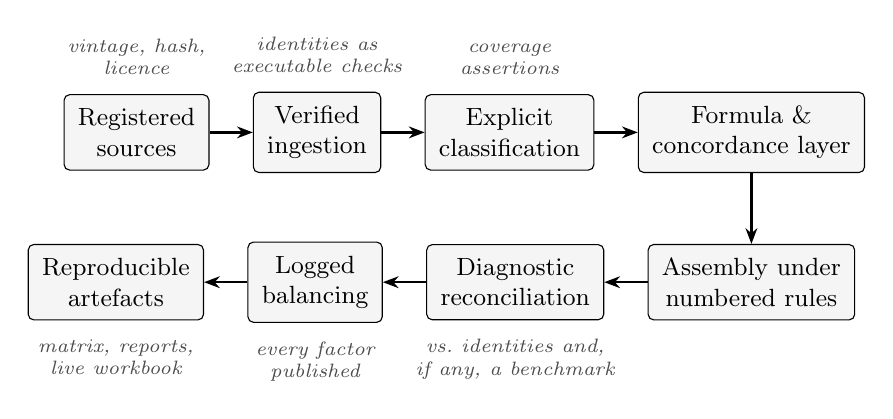
\begin{tikzpicture}[
  stage/.style={draw, rounded corners=2pt, align=center, font=\small,
                minimum height=2.2em, inner sep=5pt, fill=gray!8},
  note/.style={font=\scriptsize\itshape, text=gray!60!black, align=center},
  arr/.style={-{Stealth[length=2mm]}, thick}]
\node[stage] (s1) {Registered\\sources};
\node[stage, right=0.55cm of s1] (s2) {Verified\\ingestion};
\node[stage, right=0.55cm of s2] (s3) {Explicit\\classification};
\node[stage, right=0.55cm of s3] (s4) {Formula \&\\concordance layer};
\node[stage, below=0.9cm of s4] (s5) {Assembly under\\numbered rules};
\node[stage, left=0.55cm of s5] (s6) {Diagnostic\\reconciliation};
\node[stage, left=0.55cm of s6] (s7) {Logged\\balancing};
\node[stage, left=0.55cm of s7] (s8) {Reproducible\\artefacts};
\draw[arr] (s1) -- (s2); \draw[arr] (s2) -- (s3);
\draw[arr] (s3) -- (s4); \draw[arr] (s4) -- (s5);
\draw[arr] (s5) -- (s6); \draw[arr] (s6) -- (s7); \draw[arr] (s7) -- (s8);
\node[note, above=0.12cm of s1] {vintage, hash,\\licence};
\node[note, above=0.12cm of s2] {identities as\\executable checks};
\node[note, above=0.12cm of s3] {coverage\\assertions};
\node[note, below=0.12cm of s6] {vs.\ identities and,\\if any, a benchmark};
\node[note, below=0.12cm of s7] {every factor\\published};
\node[note, below=0.12cm of s8] {matrix, reports,\\live workbook};
\end{tikzpicture}%
}
\caption{The framework's eight stages. Auditing and construction share
the pipeline; an audit adds a comparison target at the reconciliation
stage.}
\label{fig:pipeline}
\end{figure}

\subsection{Pipeline}

The South African pipeline is twelve construction and audit scripts
(01--12) over the open toolkit; a thirteenth generates the paper's
exhibits, and scripts 14--15 implement the Kenyan and Dutch applications
of Section~\ref{sec:applications}. The design principle is that
\emph{nothing is classified by convention}. Account codes, prose
descriptions, and header labels are treated as claims to be verified,
never as facts. Concretely:

\begin{enumerate}
  \item \textbf{Ingestion with internal checks.} Readers for the supply and
  use tables recompute every embedded total and verify the layout's
  accounting identities: for each product, supply at purchasers' prices
  must equal supply at basic prices plus product taxes plus trade and
  transport margins; for each industry, output must equal intermediate
  inputs plus value added; and value added must equal the sum of its
  components---compensation of employees, other net taxes on production,
  and gross operating surplus or mixed income (coded $D1$, $D2/3$, and
  $B2/3$ in the published tables, summing to value added
  $B1$).\footnote{These are the SNA transaction codes used by Stats~SA's
  published tables: $B1$ gross value added, $D1$ compensation of
  employees, $D2/3$ other taxes less subsidies on production, $B2/3$ gross
  operating surplus / mixed income \citep{un2009sna}.} The official 2019
  tables pass all checks at a R0.5~million tolerance.
  \item \textbf{Explicit classification.} The 209 benchmark accounts are
  mapped to a canonical taxonomy (activity, commodity, factor, household,
  \ldots) in one reviewable table extracted from the workbook's own
  dictionary sheets; a coverage assertion guarantees that every account in
  the matrix is classified and nothing phantom is. Classification by prefix
  is refused by construction---for good reason, as the results show.
  \item \textbf{Concordances as data.} The 124$\to$61 industry and
  product mappings, the labour-survey industry table, and the asset and
  industry tables of the financial-statistics source are parsed from the
  benchmark's published materials into CSV concordances with completeness
  validation (every source category maps exactly once).
  \item \textbf{Institutional cells as formulas.} The technical note
  defines each macro cell in prose as a combination of SARB Quarterly
  Bulletin series. We transcribe all 46 definitions into a machine-readable
  formula table---one row per cell, holding the signed combination of
  series codes---which a small evaluator computes
  mechanically.\footnote{For example, the cell (households $\leftarrow$
  labour) is the single series KBP6240J, ``compensation of residents'';
  the cell (government $\leftarrow$ production taxes) is KBP6600J
  $-$ KBP6601J. Two rest-of-world cells that the note itself defines as
  residuals of other entries are stored as such and resolved recursively,
  e.g.\ (rest of world $\leftarrow$ labour) $=$ (labour income) $+$
  (labour from abroad) $-$ (labour to households).} The one unpublished
  input enters this table as a flagged parameter evaluated under two
  scenarios: \emph{as built} (the benchmark's value) and \emph{public
  proxy} (the closest published series), so that its effect is measured
  rather than absorbed.
  \item \textbf{Share systems from microdata.} Capital-type shares from the
  AFS PPE schedules; occupational wage-bill shares from LMD 2018--2019
  (weighted employment $\times$ average wage, national occupation wage for
  empty cells, two-year averaging); household groups as weighted
  expenditure deciles with the top decile in five 2\,per\,cent bands from
  the LCS.
  \item \textbf{Assembly under numbered rules.} The full 209-account SAM is
  assembled from the above; every point where the benchmark's choice is
  unpublished or undocumented is replaced by an explicit rule, numbered
  R1--R7 and reproduced in Appendix~\ref{app:rules},\footnote{The rules
  also ship as part of the replication package and are printed on a
  dedicated sheet of the generated workbook.} so that the difference
  between our SAM and the benchmark is, by construction, the union of
  disclosed rules.
  \item \textbf{Balancing with a log.} Residual imbalances---confined to
  the household income block---are closed by RAS with fixed payer totals
  and group outlay targets; the implementation refuses negative seeds,
  reports convergence, and returns the multiplicative factor of every
  adjusted cell, which is published in the workbook.
\end{enumerate}

\subsection{Audit method: reconciliation and recovery}

The audit compares each constructed block with the benchmark at the finest
common level and treats any discrepancy as a diagnostic object. Three
patterns recur. \emph{Identity-guided attribution}: a mismatch is traced by
asking which accounting identity it violates and what movement would repair
it (this is how mislabelled accounts and valuation mismatches announce
themselves). \emph{Grid recovery}: when documentation is silent over a
small discrete choice set---which source edition, which measurement column,
which signs---we evaluate all candidates against the benchmark and accept a
choice only if it is uniquely best, reporting the
margin.\footnote{Two instances matter below. For one aggregation formula,
the six quoted series were each allowed a coefficient of $-1$, $0$, or
$+1$; of the $3^6 = 729$ combinations, exactly one reproduces the
benchmark, and the runner-up misses by R2.5~billion. For the capital-stock
split, the grid crossed the source's two published editions (2019
preliminary versus 2019 revised) with two candidate stock measures
(opening versus closing carrying value); ``recovering the vintage and
measure'' means identifying which edition--measure pair the benchmark
used.} \emph{Scenario pricing}: where an input is genuinely non-public, we
quantify the cost of its best public substitute rather than absorb it
silently.

\section{Results}\label{sec:results}

Table~\ref{tab:headline} summarises the audit in the metrics that matter
for reproducibility; the subsections unpack each row. One remark applies
throughout: none of the findings below is a criticism of the benchmark's
authors, whose documentation is far above the norm for the genre and whose
distributed workbook is what made a cell-level audit possible at all. Small
reconciling interventions are a normal and necessary part of SAM
compilation; our findings concern whether the record allows them to be
seen, not whether they should exist.

\begin{table}[t]
\centering\small
\caption{Headline replication metrics: our reconstruction from
publicly obtainable sources, audited against the published benchmark.
Comparisons use the tolerance of Section~\ref{sec:method:terms}
(R0.5~million, the benchmark workbook's rounding grain) unless stated;
``comparable'' cells are those nonzero in both our matrix (6{,}779
nonzero cells) and the benchmark's (6{,}737).}
\label{tab:headline}
\begin{tabularx}{\textwidth}{lXl}
\toprule
Block & Metric & Result \\
\midrule
Production (61 activities) & output, intermediates, prod.\ taxes, VA & exact ($\le$R0.5m), 61/61 each \\
Final demand (5 categories) & per-commodity agreement & exact, all commodities (316/316) \\
Institutional macro (SARB) & 45 computable cells & 43 exact; 45 within 1\%; max 0.139\% \\
Capital split (6 types) & activity--type shares & median 0.18pp; 73.6\% within 1pp \\
Occupation split (10) & activity--occupation shares & median 0.04pp; 88.7\% within 1pp \\
Household groups (14) & wage-income anchor & mean 0.74pp; max 1.9pp \\
Full matrix (209 accounts) & 6{,}732 comparable cells & 62.5\% equal within R0.5m \\
Balanced SAM (v0.2) & max account imbalance & R7m; RAS factors in $[0.907, 1.143]$ \\
\midrule
Non-public inputs & count; priced effect of proxy & 1; mtx $+16.1$\%, stx $-1.5$\% \\
Divergences (record vs.\ data) & catalogued in five classes & 8 (Sec.~\ref{sec:discussion}; App.~\ref{app:evidence}) \\
\bottomrule
\end{tabularx}
\end{table}

\subsection{The production and commodity blocks reproduce exactly}
\label{sec:results:production}

Aggregating the official supply and use tables through the published
concordances reproduces the benchmark's production side to within
R0.5~million on \emph{all} 61 activities: gross output, intermediate
consumption, production taxes, and value added at factor cost each deviate
by 0.0000\,per\,cent. Final demand reproduces exactly per commodity in
every category (households 93/93 commodities, government 3/3,
exports 97/97, fixed capital formation 21/21, and
inventories-plus-residual 102/102---316/316 in all,
confirming that the benchmark's stock-change account absorbs the use
table's residual column). The benchmark matrix itself is exactly balanced
(maximum $|$row$-$column$|$ gap below R0.001~million across the 210
accounts of its distributed matrix; the comparison below is on the 209
accounts of our rebuild). For the macro comparison of
Section~\ref{sec:results:macro} the benchmark is aggregated to the
technical note's Table-2 accounts, the margin account consolidating away
exactly.

Three discrepancies had to be resolved to get there, and each is a finding
about naming rather than about numbers. The account \texttt{atx} carries an
activity-style prefix but is taxes on production (it equals the use table's
$D2/3$ exactly on 61 of 61 activities); the accounts \texttt{cler} and
\texttt{craf} carry the commodity prefix but are the clerical and craft
\emph{occupation} accounts---before reclassification they masquerade as a
systematic R479~billion overstatement of intermediates spread across every
activity; and the value-added comparison closes only at factor cost, since
the benchmark parks production taxes outside its factor payments. The
workbook's own dictionary sheet later confirmed all three
identifications---and added a fourth: the descriptions of the capital
accounts \texttt{mach}, \texttt{nitc}, and \texttt{trnp} are rotated by one
position relative to the technical note's authoritative list.

\subsection{The institutional macro block from SARB series}
\label{sec:results:macro}

Evaluating the technical note's 46 macro cell formulas over the December
2022 SARB Quarterly Bulletin series reproduces 43 of the 45 computable
cells exactly; all 45 are within 1\,per\,cent and the largest deviation is
0.139\,per\,cent. (Of the 46 cells, 43 evaluate directly from KBP-series
formulas and two are defined residually from the others---together the 45
``computable'' cells---while the 46th depends on the unpublished customs
input priced below.) Getting there required three corrections that are
themselves results:

\begin{itemize}
  \item \textbf{A garbled formula, uniquely recovered.} No signed
  combination of the six series quoted for the intra-enterprise cell
  reproduces the benchmark. Searching all $3^6$ coefficient vectors in
  $\{-1,0,1\}$ yields exactly one exact solution---with different signs than
  the prose and one quoted series unused---and the next-best candidate
  misses by R2.5~billion.
  \item \textbf{The unpublished input, priced.} The product-tax cells
  subtract the benchmark's unpublished customs figure (R48{,}934m), not the
  public series the note cites (KBP4590J, R56{,}805m); the note itself
  prints both variants in different places. Under the public proxy, import
  duties deviate by $+16.1$\,per\,cent and product taxes by
  $-1.5$\,per\,cent---the total measured cost, in this SAM, of its one
  non-public input.
  \item \textbf{An unrecorded reconciling adjustment.} Twin gaps of exactly
  $-$R596~million appear in the two government--enterprise cells. A
  data-revision explanation is tested and set aside (the June and December
  2022 bulletins carry identical values for every series involved). Adding
  $+596$ to both directions of a bilateral flow is the unique minimal edit
  that preserves both accounts' balances, so the pattern is consistent with
  a routine reconciling adjustment made during compilation and not recorded
  in the note---exactly the kind of small, legitimate intervention that
  cell-level provenance would turn from a discovery into a declaration.
\end{itemize}

Table~\ref{tab:macro} reports the cells where these three findings act,
under both scenarios; all other computable cells are exact.

\begin{table}[t]
\centering\small
\caption{Institutional macro cells requiring correction or judgment
(R~million; deviations against the benchmark). ``Proxy'' replaces the
unpublished customs figure with the public series KBP4590J.}
\label{tab:macro}
\begin{tabular}{llrrrr}
\toprule
Entry & Cell (receiver $\leftarrow$ payer) & Computed & Benchmark & Dev.\ \% & Proxy dev.\ \% \\
\midrule
vi & stx $\leftarrow$ commodities & 519,805 & 519,805 & +0.00 & -1.51 \\
vii & mtx $\leftarrow$ commodities & 48,934 & 48,934 & +0.00 & +16.09 \\
xv & enterprises $\leftarrow$ enterprises & 857,644 & 857,644 & +0.00 & +0.00 \\
xvii & government $\leftarrow$ enterprises & 428,816 & 429,412 & -0.14 & -0.14 \\
xxviii & enterprises $\leftarrow$ government & 686,931 & 687,527 & -0.09 & -0.09 \\
xxxiv & government $\leftarrow$ stx & 519,805 & 519,805 & +0.00 & -1.51 \\
xxxv & government $\leftarrow$ mtx & 48,934 & 48,934 & +0.00 & +16.09 \\
\midrule
\multicolumn{6}{l}{\emph{Remaining 39 cells: exact (43 of 45 computable within 0.01\%)}} \\
\bottomrule
\end{tabular}

\end{table}

\subsection{Share systems: recovery and honest residuals}
\label{sec:results:shares}

\textbf{Capital.} The technical note specifies neither the AFS edition nor
the stock measure behind its six-way capital split. Grid-testing editions
$\times$ carrying-value columns leaves \emph{2019 revised, closing
values} as the only candidate in the grid consistent with the benchmark
(median share deviation 0.18~percentage
points; 73.6\,per\,cent of activity--type shares within 1pp), against
0.72pp for the preliminary edition that the AFS 2019 publication page
supplies by default. Residual outliers are concentrated and interpretable:
posts and telecommunications deviates by up to 34pp on network equipment,
consistent with a sector-specific reclassification made during compilation
and not reported in the note; and six
activities (agriculture, education, financial intermediation, insurance,
public administration, non-observed) are absent from the AFS altogether, so
their published splits rest on undocumented sources.

Table~\ref{tab:grid} shows the recovery grid.

\begin{table}[t]
\centering\small
\caption{Grid recovery of the capital split's undocumented basis: agreement
with the benchmark's activity--type shares by AFS edition and stock
measure.}
\label{tab:grid}
\begin{tabular}{llrr}
\toprule
AFS edition & Stock measure & Median $|$diff$|$ (pp) & Within 1pp (\%) \\
\midrule
2019 preliminary & opening & 1.05 & 49.1 \\
2019 preliminary & closing & 0.72 & 57.9 \\
2019 revised & opening & 0.72 & 58.2 \\
2019 revised & closing $\leftarrow$ recovered & 0.18 & 73.6 \\
\bottomrule
\end{tabular}

\end{table}

\textbf{Occupations.} Implementing the note's wage-bill procedure on the
LMD microdata reproduces the benchmark's $10\times61$ occupation shares
with median deviation 0.038pp (mean 0.86pp; 88.7\,per\,cent of 610 shares
within 1pp; maximum 24pp in two small-sample industries). A methodological
aside earns its keep here: our own first pass silently dropped the
private-households industry---6{,}202 observations and the home of the
domestic-worker occupation---because a parser assumed three-digit industry
codes. The pipeline's coverage assertion caught it; conventions failed
symmetrically on both sides of the audit.

\textbf{Households.} Two dictionary-free anchors test the benchmark's
group definition, and they disagree---informatively. The wage-income
anchor identifies \emph{household-level} expenditure deciles (top decile
in five 2\,per\,cent bands): under that definition the LCS wage-income
distribution matches the benchmark's labour-to-household block at mean
0.74pp (max 1.9pp), while per-capita grouping fits markedly worse (mean
1.8pp, max 7.9pp). The consumption anchor cannot corroborate it: it fits
poorly under the household-level grouping (up to 5.9pp) and in fact sits
closer to the per-capita alternative (mean 0.71pp against 1.46pp). The
note itself explains why the consumption block is uninformative here: its
consumption shares were carried over from an earlier SAM rather than
recomputed from the LCS---inherited provenance that a fresh, documented
build cannot and should not reproduce, and that decouples the consumption
pattern from whichever grouping the income side uses. The identification
therefore rests on the wage anchor alone.

Table~\ref{tab:occ} details the occupation system by occupation, and
Figure~\ref{fig:ecdf} plots the full distribution of share deviations for
the two microdata-based systems: the mass of both distributions sits far
below one percentage point, with thin, interpretable tails.

\begin{table}[t]
\centering\small
\caption{Occupation shares versus the benchmark, by occupation
(deviations in percentage points across 61 activities).}
\label{tab:occ}
\begin{tabular}{lrrr}
\toprule
Occupation & Median $|$diff$|$ (pp) & Max (pp) & Within 1pp (of 61) \\
\midrule
Managers & 0.340 & 19.02 & 42 \\
Professionals & 0.068 & 24.40 & 50 \\
Technicians & 0.065 & 16.13 & 53 \\
Clerks & 0.080 & 14.94 & 53 \\
Service and sales & 0.028 & 10.01 & 54 \\
Skilled agriculture & 0.000 & 0.84 & 61 \\
Craft & 0.061 & 17.26 & 55 \\
Plant/machine operators & 0.063 & 10.27 & 55 \\
Elementary & 0.087 & 22.81 & 58 \\
Domestic workers & 0.000 & 1.28 & 60 \\
\bottomrule
\end{tabular}

\end{table}

\begin{figure}[t]
\centering
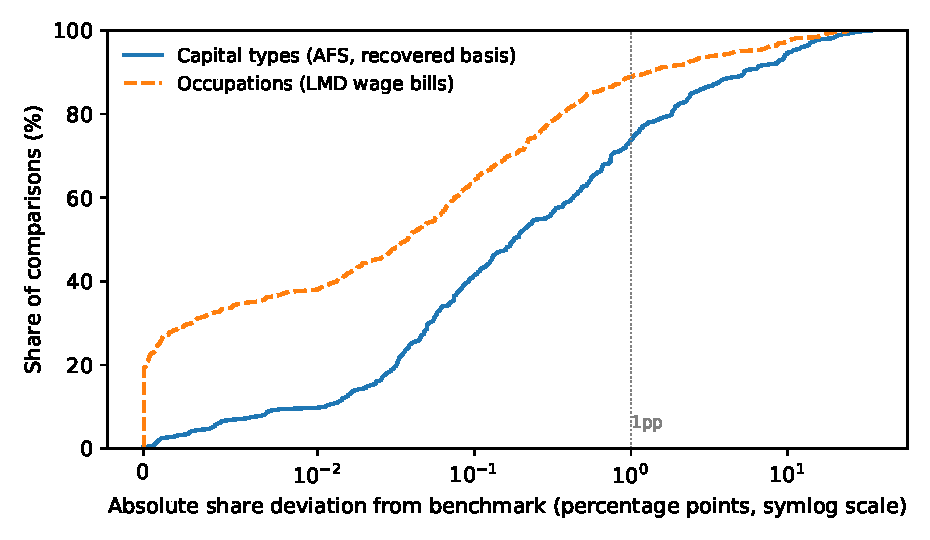
\includegraphics[width=.92\textwidth]{figures/fig_share_ecdf}
\caption{Cumulative distribution of absolute share deviations from the
benchmark for the capital-type and occupation systems.}
\label{fig:ecdf}
\end{figure}

\subsection{Assembly and balancing}
\label{sec:results:assembly}

Assembling the full 209-account SAM from our registered inputs under
seven numbered rules yields 6{,}779 nonzero cells. Of these, 6{,}732 are
\emph{comparable}---nonzero in both our matrix and the benchmark's (which
has 6{,}737)---and 62.5\,per\,cent of the comparable cells equal the
benchmark within the R0.5~million tolerance: the entire production and
commodity side.
Every material imbalance lies in the 14 household groups (maximum
R100~billion, 2.0\,per\,cent of value added at the ninth decile): precisely
the footprint of the proxy distribution rules, since group-specific income
composition is the one place our obtainable inputs are coarser than the
benchmark's item-level survey work. Balancing the household income block by
RAS---payer totals and group outlays held fixed as documented targets---
closes the household imbalance to R0.06~million with adjustment factors
confined to $[0.907, 1.143]$, leaves every other account within
R7~million---under 0.0002\,per\,cent of GDP, and the sense in which
``balanced'' is used throughout---and moves the block slightly
\emph{toward} the benchmark's item-based values. The result, SAM v0.2, ships as a workbook whose totals and balance
checks are live formulas and whose 266 balancing factors are printed on
their own sheet.

\section{Two further applications: the replicability spectrum}
\label{sec:applications}

The South African audit is the framework's deep case, but a method whose
value is generality must be shown doing different jobs under different data
regimes. This section applies it twice more, at the two ends of the public
data spectrum. In Kenya, where the machine-readable supply--use detail
behind the country's leading SAM is not published, the framework
establishes what \emph{can} be verified from public aggregates---and shows
exactly where verification must stop. In the Netherlands, where complete
harmonised tables are a single API call away, the framework runs in the
opposite direction: not auditing an existing SAM but \emph{generating} one,
with no benchmark consulted at any point. Together with South Africa the
three cases trace a replicability spectrum that we argue is the right way
to think about SAM infrastructure worldwide.

\subsection{Kenya: auditing at the aggregate boundary}
\label{sec:applications:kenya}

The most widely used Kenyan SAM is IFPRI's 2019 Nexus matrix
\citep{thurlow2021}, distributed as an open CC-BY dataset. Its
construction, like that of the Nexus programme generally, reconciles
scattered sources by cross-entropy estimation \citep{robinson2001}, so
cell-level replication of the kind achieved for South Africa is not the
relevant test: a CE-reconciled matrix is a model output, and the honest
question is what its public record allows an outsider to verify. The
framework's answer has three layers.

\emph{Structure verifies.} The distributed file parses into 108 accounts
whose groups (42 activities, 42 commodities, five factors, ten
representative households, and the transaction-cost, enterprise,
government, tax, accumulation, and external accounts) match the data
paper's stated design exactly. The matrix balances only to the file's own
integer rounding---values are printed in whole Sh billions, and account
imbalances reach Sh~5~billion---which is itself a small finding about
distribution practice: rounding a balanced matrix unbalances it.

\emph{Macro controls verify approximately, and the deviations are
informative.} Table~\ref{tab:kenya} compares the SAM's implied national
aggregates with the published current-price tables of the KNBS Economic
Survey 2020. The production side sits a uniform 1.0\,per\,cent below the
published figures---GVA, product taxes, and GDP all shifted
together---which is the signature of a vintage difference in the
then-provisional 2019 accounts, not of a methodological choice
(Section~\ref{sec:discussion}'s class~3). Fixed capital formation,
inventories, and imports agree essentially exactly. The large deviations
are concentrated in private consumption ($-9.2$\,per\,cent), government
consumption ($+9.1$\,per\,cent), and exports ($+13.6$\,per\,cent), and
they have a structural explanation: KNBS's own expenditure table carries a
production-versus-expenditure discrepancy of Sh~$-352$~billion
(3.6\,per\,cent of GDP), and a balanced SAM cannot carry a statistical
discrepancy---the reconciliation \emph{must} allocate it somewhere. The
deviation pattern is consistent with the discrepancy, together with
associated source and definitional differences, being absorbed primarily
through the consumption and trade aggregates; aggregate comparisons
cannot identify the allocation uniquely, and that very limit is the
point. Nothing in the public record documents the allocation at the
level where it acts, which is precisely the provenance gap the paper's
proposal addresses.

\begin{table}[t]
\centering\small
\caption{Kenya: the IFPRI 2019 Nexus SAM against published KNBS controls
(Sh billion, current prices; Economic Survey 2020, Tables 2.1 and 2.7,
2019 provisional).}
\label{tab:kenya}
\begin{tabular}{lrrr}
\toprule
Aggregate & SAM & KNBS & Dev.\ \% \\
\midrule
GVA (all activities) & 8,825 & 8,912 & -1.0 \\
Taxes on products & 821 & 829 & -0.9 \\
GDP at market prices & 9,646 & 9,740 & -1.0 \\
Private consumption (incl. NPISH) & 7,295 & 8,035 & -9.2 \\
Government consumption & 1,387 & 1,271 & +9.1 \\
Gross fixed capital formation & 1,631 & 1,632 & -0.1 \\
Changes in inventories & 63 & 63 & -0.2 \\
Exports of goods and services & 1,331 & 1,172 & +13.6 \\
Imports of goods and services & 2,071 & 2,082 & -0.5 \\
Statistical discrepancy & 0 & -352 & --- \\
\bottomrule
\end{tabular}

\end{table}

\emph{Cell-level audit is bounded by publication practice, not by
method.} The SAM's supply--use core descends from KNBS's 2009 benchmark
tables, whose full balanced database (151 products by 81 industries) is,
per the Economic Survey, available from KNBS on request but published only
as condensed print tables. We did not request it, and the boundary tested
here is therefore a specific one: what an auditor can verify from the
public record alone, without privileged access or correspondence with the
producer. That is the boundary a reader of a published SAM faces, and the
one the paper's standards proposal addresses; an audit conducted on
requested files would test a different and more permissive question. Two
consequences follow. The Kenyan evidence below is confined to structure,
grain, and macro controls---the depth the public record supports---and the
claim that the South African pipeline would extend to the Kenyan detail
remains untested: the reader for the KNBS layout, and its concordances,
would still have to be written, even though the method behind them is
unchanged. That boundary---audit feasible in principle, unreachable from
what is published---defines the middle of the replicability spectrum.

\subsection{The Netherlands: benchmark-free generation}
\label{sec:applications:nl}

The third application inverts the exercise. For a country inside the
European statistical system, the framework should need no benchmark, no
technical note, and no manual acquisition: the ESA transmission programme
puts harmonised supply--use tables and sector accounts on a public API
\citep{eurostat2008}. We test that claim on the Netherlands for 2019.
Three API calls retrieve the supply table, the use table, and the full
sequence of non-financial sector accounts (about 180~KB in total); a
70-line JSON-stat reader added to the toolkit decodes them, and a single
script assembles a macro accounting matrix and balances it into a macro
SAM. No published SAM was consulted at any point during construction or
validation---though, as the results below make clear, that is a statement
about SAMs and not a claim of independent verification: the checks
available here are internal consistency and agreement with published
national-accounts aggregates drawn from the same compilation system that
supplies the inputs.

Two results follow. First, \emph{the official tables are internally
exact}: every identity the toolkit enforces---output and value-added
identities for all 65 industries, the import identity, and the
supply--demand balance of all 65 products---closes at a EUR~1~million
tolerance with zero findings. The contrast with the audit cases is the
point: when a statistical office publishes machine-readable tables under a
harmonised standard, deterministic verification is free. Even here,
however, the framework's refusal to classify by convention earned its
keep: Eurostat's category lists mix aggregates with overlapping
sub-details (NACE section codes alongside their own divisions), and a
na\"ive selection double-counts; the toolkit's coverage-based partition,
guarded by an assertion that the chosen codes tile the total exactly,
caught both this and a code collision between the NACE section~P
(education) and the ESA transaction P-codes. Names mislead in Luxembourg
as in Pretoria.

Second, \emph{the generated matrix closes to within 1.5\,per\,cent of
GDP with every residual attributed---and a logged balancing step then
closes it exactly}. We are careful with terminology here: a SAM is
defined by every account balancing, so the direct output of the
generation---the 18-account \emph{macro accounting matrix}---is the
diagnostic product, and the SAM is what balancing makes of it. The matrix
routes factor income, taxes, transfers, and the ESA bridging items (the
pension-fund adjustment D8, capital transfers D9, net lending B9, and the
residents-abroad consumption adjustments) through explicit instrument
accounts; GDP at basic prices emerges at EUR~724{,}960~million, on the
published figure, and compensation of employees closes to the euro across
four series. Both agreements are internal to the Dutch national accounts:
the four series and the published aggregate are outputs of one compilation
system, so what they establish is that our assembly preserves CBS's own
consistency, not that it is independently corroborated. Table~\ref{tab:netherlands} reports the residual
of every account before balancing: twelve are exactly zero, and the six
that are not are all below 1.5\,per\,cent of GDP and attach to known ESA
boundary items (the domestic-versus-national concept in compensation,
mixed-income attribution, capital-account detail). Consistent with the
framework's first commitment, the residuals are published, not hidden;
the balanced macro SAM is then produced by the toolkit's logged RAS
step: it converges to a maximum residual below EUR~0.01~million at full
precision, with all 70 adjustment factors inside $[0.9832, 1.0282]$,
concentrated on the rest-of-world cells---exactly where the attributed
residuals sat---and every factor ships with the matrix. One caveat
applies to the distributed artefact, and it is the same one this paper
notes for the Kenyan file: the CSV prints values at EUR~0.1~million
precision, so recomputing account residuals from the distributed file
yields rounding imbalances of up to EUR~0.2~million; the full-precision
matrix regenerates from the replication package. The balancing choices (the treatment
of two negative cells, the target vector, and the choice of RAS), the
invariants they preserve, and a target-vector sensitivity check are
documented in Appendix~\ref{app:nlbalance}.

\begin{table}[t]
\centering\small
\caption{Netherlands: account residuals of the generated 2019 macro
accounting matrix, before balancing (no benchmark consulted; GDP at basic
prices EUR 724{,}960m). The logged RAS step closes all residuals with
adjustment factors in $[0.9832, 1.0282]$.}
\label{tab:netherlands}
\begin{tabular}{lrr}
\toprule
Account & Residual (EUR m) & \% of GDP \\
\midrule
Corporations & +1,532 & +0.21 \\
Government & +1,443 & +0.20 \\
Households & +9,111 & +1.26 \\
Labour & -4,193 & -0.58 \\
Rest of world & -10,830 & -1.49 \\
Savings--investment & +2,937 & +0.41 \\
\midrule
\multicolumn{3}{l}{\emph{Remaining 12 accounts (production, taxes, capital, instruments): residual zero}} \\
\bottomrule
\end{tabular}

\end{table}

The cost ledger deserves its own sentence, because it carries the paper's
economic claim. The South African reconstruction required four public
providers, a registered microdata access, and bulk downloads diagnosed
around a broken online query system; the Kenyan case required locating
condensed print tables inside a 322-page yearbook; the Dutch case required
three API calls and a single working session, and the 70-line reader that
enabled it works unchanged for every country in the ESA transmission
programme. Out-of-sample runs for Austria and Poland confirm that the
generator transfers---and that confidentiality suppression remains a
cell-level constraint even under harmonised publication;
Appendix~\ref{app:transfer} reports the results. Conditional on the
toolkit, the marginal implementation effort for a verified macro SAM is
therefore shaped largely by the accessibility and structure of the
published data---the replicability spectrum restated as effort.

\section{Discussion}\label{sec:discussion}

\subsection{A taxonomy of divergence between record and artefact}

Set side by side, the audit's findings sort into five classes, and it is
worth stating plainly that every reported finding was \emph{first
detected} by arithmetic---an identity refusing to close, a grid search
returning a unique survivor---and only then interpreted against the
source record (Appendix~\ref{app:evidence} states each finding's
evidentiary status):

\begin{enumerate}
  \item \textbf{Names mislead.} Account codes mislabel their contents
  (\texttt{atx}, \texttt{cler}, \texttt{craf}); dictionary descriptions
  rotate against their codes (\texttt{mach}/\texttt{nitc}/\texttt{trnp}).
  Any pipeline that classifies by prefix or label inherits these slips
  silently; ours refuses to, and both of the audit's largest apparent
  anomalies (R479~billion of phantom intermediates; a 125\,per\,cent
  value-added ``error'') dissolved into classification fixes.
  \item \textbf{Prose diverges from data.} A formula's printed signs do not
  reproduce the matrix they describe; the same cell is printed with two
  different values in two places. The data adjudicate.
  \item \textbf{Vintages drift.} The default download of a source (AFS 2019
  preliminary) is not the edition actually used (2019 revised); nothing in
  the record says so, and only a grid test can tell.
  \item \textbf{Inputs are unavailable.} One input is unpublished; its
  effect ($+16.1$\,per\,cent on import duties under the public proxy) is
  invisible until priced.
  \item \textbf{Adjustments go unrecorded.} A symmetric R596~million
  reconciling edit balances two accounts and appears nowhere in the record;
  inherited consumption shares import a different survey vintage's
  processing into a matrix whose documentation implies otherwise.
\end{enumerate}

To repeat the point made in Section~\ref{sec:results}: these are properties
of the \emph{medium}---prose describing spreadsheets---not of the authors,
whose record-keeping is far better than the norm. That is precisely what
makes the count suggestive: if the best-documented SAM in its class
carries five classes of silent divergence between record and artefact,
there is little reason to expect fewer in matrices published with no
dictionary, no formula note, and no distributed cell-level file---and for
those, the audit reported here could not even be attempted, because its
first step is a distributed matrix to compare against. One deep audit
cannot establish a distribution over the population of SAMs, and we do not
claim it does; what it establishes is that the divergences are not
hypothetical, and that detecting them required a machine-readable record
that most published SAMs do not supply.

The two further applications confirm that the taxonomy travels. Kenya
exhibits class~3 (the SAM's production side sits a uniform 1.0\,per\,cent
from the Economic Survey print, the signature of a provisional-accounts
vintage) and class~5 at national scale (the accounts' own
3.6-per-cent-of-GDP discrepancy is absorbed by the reconciliation with no
cell-level record of where). The Netherlands, with the cleanest data of
the three, still exhibits class~1: Eurostat's mixed-granularity category
lists and a NACE/ESA code collision would silently double-count under
prefix-based selection, and were caught only by the toolkit's tiling
assertion.

\subsection{From audit to construction workflow}
\label{sec:discussion:workflow}

The framework is not only a microscope; it is a factory. The same pipeline
that audits the benchmark \emph{builds} a SAM: scripts ingest and verify
the official tables, assemble the production and commodity blocks
mechanically, compute the institutional cells from published series,
apply survey-based share systems, and balance the result with a logged
adjustment. What remains for the economist is exactly the residue that
identities and obtainable data cannot determine---in this application, the
customs split, six sectors' capital shares, and the distributional detail
of household income. That inversion is the practical payoff: expert
attention stops being spread across ten thousand spreadsheet cells and
concentrates on the handful of judgments that genuinely require it, each
of which the framework forces into the open as a numbered rule. Updating
the matrix for a new benchmark year, or transferring it to a country with
comparable sources, reuses everything except those judgments.

\subsection{Implications: a standards proposal}
\label{sec:discussion:standards}

Two practices would have made most of this paper's detective work
unnecessary, and both are cheap. We state them as a proposal for producers
of SAMs---statistical offices, research institutes, and international
programmes alike:

\begin{enumerate}
  \item \textbf{Publish cell-level provenance.} Each cell of a released SAM
  should carry its source series, transformation, and any manual
  adjustment. The R596~million edit and the inherited consumption shares
  would then be declarations rather than discoveries, and reconciling
  interventions---a normal part of compilation---would be visible instead
  of latent.
  \item \textbf{Publish machine-readable construction rules.} The
  benchmark's technical note was nearly a program; had it been an actual
  one (as our transcribed formula table now is), the sign discrepancy could
  not have survived contact with the data, and replication would be a
  command rather than a project. Concordances, account dictionaries, and
  balancing targets belong in the same release.
\end{enumerate}

Neither requires changing a single methodological choice, and both are
by-products of building the matrix in code to begin with. Our toolkit is
offered as working infrastructure for exactly that: an open reference
implementation of registered sources, executable identities, explicit
classification, formula tables, diagnostic balancing, and workbook
generation, intended to be reused wholesale for other countries and years.

\subsection{Cost: a three-country ledger}

We report the development ledger factually and claim nothing causal about
labour saving from it. The South African case required registering
sources from four providers, one registered microdata access, and bulk
downloads worked around a non-functioning online query system; the Kenyan
case required locating condensed print tables inside a 322-page yearbook;
the Dutch case required three API calls and roughly 300 new lines of code
(70 of them a reader that now serves every ESA-transmitting country). The
claim we do make is conditional and testable: the marginal cost of the
\emph{next} SAM built on the toolkit is largely the cost of its
country-specific concordances and share systems, and the Dutch
application is a first operational indication of that claim at the macro
level. Across the three cases, publication format emerges as a major
determinant of marginal implementation effort---which is what the
standards proposal above is for.

\subsection{Limitations}

The deep audit inherits its benchmark's scope---one country, one year, one
SAM family---and the two further applications, while they demonstrate
transfer, are deliberately shallower: Kenya stops at structure and macro
controls because the machine-readable detail is not public, and the Dutch
exercise generates and balances a macro SAM, not a full multi-sector SAM with
distributional detail (that extension is mechanical for the production
core, which the API supplies at 65 industries, but household disaggregation
would require the national budget-survey work the South African case
illustrates). Six activities' capital splits and the item-level detail of the
household systems remain beyond the inputs we hold, and our
balanced household block is a disciplined proxy, not a reconstruction---
closing that gap requires the survey's item-level classifications, which
are obtainable and queued. The recovered choices (editions, measures,
signs) are unique within their tested grids, not proofs of intent; where
no grid candidate fits exactly---as in the capital split---the true basis
may lie outside the set we enumerated.

Two limits are structural rather than circumstantial, and neither is
removed by better data. The first concerns what the method is able to
detect. Every finding reported here was identified because it left an
arithmetic trace: an identity that did not close, a grid search returning
a single survivor, or a pair of gaps whose symmetry was unlikely to be
coincidental. Divergences that leave no such trace pass through this
framework without being detected. These include compensating errors,
adjustments that happen to land on a plausible value, and errors shared
between the artefact and the sources against which it is checked. The
audit therefore establishes that a matrix is reproducible from its stated
record, which is a narrower property than correctness. The comparison in
Section~\ref{sec:results:jrc} narrows this gap without closing it: an
independently constructed SAM for the same country-year agrees with ours
on every macro aggregate to within 0.8~per~cent, which is meaningful
corroboration, but it remains agreement between two constructions resting
on a shared official source rather than a second measurement of the same
economy. An error contained in the source record itself would not be
detected by any check reported here.

The second limit is that the framework records without evaluating. It
reports every adjustment factor, coverage share, and residual, but it
does not encode a threshold above which a matrix should be rejected, and
we do not propose one. The tolerable magnitude of a balancing adjustment
depends on the account, the country, and the intended use of the SAM, so
a threshold calibrated to three cases would carry more apparent authority
than the evidence supports. What the framework changes is the
availability of the question rather than its answer: because the factors
and residuals are published, a reader can apply whichever threshold their
application requires. Rejection criteria for the field would need to be
agreed among producers rather than set by a single implementation.

Finally, our own pipeline's mistakes---one of which we document---were
caught by the same assertions we advocate; we take that as the strongest
available evidence for building them in.

\section{Conclusion}\label{sec:conclusion}

A national social accounting matrix can be rebuilt from publicly
obtainable sources---in
this application, Statistics South Africa's supply and use tables and
Annual Financial Statistics, the South African Reserve Bank's Quarterly
Bulletin series, and the Labour Market Dynamics and Living Conditions
surveys---with its production and commodity structure exact, its
institutional macro structure exact up to one priced unpublished input and
one discrepancy consistent with an unrecorded adjustment, and its
distributional detail
approximated within disclosed limits and closed by biproportional (RAS)
balancing whose every factor is logged. The exercise yields a balanced,
fully regenerable SAM; a catalogue of divergences between record and
artefact, each first detected by deterministic reconciliation and then
interpreted against the source record; and an open toolkit offered as
reproducible infrastructure for official SAM construction. The same
framework, unchanged, audits Kenya's leading SAM to the boundary its
publication format imposes---verifying structure and macro controls, with
a deviation pattern consistent with the accounts' own statistical
discrepancy being absorbed through consumption and trade---and generates
a Dutch macro accounting matrix from three API calls with no benchmark at
all, every residual attributed, then balances it into a SAM with every
adjustment factor logged. The three cases are one argument: SAM
construction can move from an opaque artisanal exercise to an auditable,
executable statistical-production process, and what separates an exactly
replicable SAM from an unauditable one is not method, geography, or
income level, but whether the underlying tables are published
machine-readably and whether construction choices are recorded where they
act. The idea worth carrying away is therefore the
simple one the evidence keeps confirming: cell-level provenance and
machine-readable construction rules, published alongside every SAM, would
make such audits---and such SAMs---routine. The immediate next steps are
the survey item-level household systems, cross-entropy balancing as an
alternative adjustment principle, and extending the Dutch generation to a
full multi-sector SAM across the ESA-transmitting countries.

\section*{Reproducibility and AI disclosure}\label{sec:disclosure}
\addcontentsline{toc}{section}{Reproducibility and AI disclosure}

The replication package comprises fifteen scripts over an open toolkit
(\texttt{edikit}, released under the Apache-2.0 licence)---the South
African construction and audit pipeline, the exhibit generator, and the
Kenyan and Dutch applications---plus a source registry with SHA-256 hashes
for every input, derived concordances and formula tables, per-script
validation reports, and a workbook whose totals and balance checks are
live formulas. All results in this paper regenerate from
the registered sources. Survey microdata are used under DataFirst access
conditions and are not redistributed---only aggregated shares appear in any
output. The package is openly available at
\url{https://github.com/kodzovee9/tekmeris} and archived at
\href{https://doi.org/10.5281/zenodo.21419195}{doi:10.5281/zenodo.21419195};
Appendix~\ref{app:toolkit} maps each of the paper's claims
to the script that produces it and the validation report that records
it.

The toolkit and the computations reported here were prepared with use of
a large language model (Anthropic's Claude) for code generation and
diagnosis. No AI-generated number
enters any result without passing the pipeline's accounting identities
and coverage assertions; all generated code, mappings, and outputs were
reviewed by the author, who assumes full responsibility for the results.
The paper reports one instance (Section~\ref{sec:results:shares}) where
those assertions caught an AI-introduced error---which we regard as the
safeguards working as designed.


\bibliographystyle{apalike}
\bibliography{references}

\appendix
\section{Disclosed construction rules}\label{app:rules}

Table~\ref{tab:rules} reproduces the numbered rules under which our SAM
departs from the benchmark's (unpublished or unrecorded) choices. Each rule
is implemented in the replication package and printed in the generated
workbook; ``measured consequence'' refers to the comparison against the
benchmark reported in Section~\ref{sec:results}.

\begin{table}[h]
\centering\small
\caption{Rules R1--R7: explicit substitutes for non-public or unrecorded choices.}
\label{tab:rules}
\begin{tabularx}{\textwidth}{lXX}
\toprule
Rule & Construction & Replaces / measured consequence \\
\midrule
R1 & Import duties by commodity: total from the public series KBP4590J, allocated by import shares & Unpublished customs data; $+16.1$\% on import duties \\
R2 & Other product taxes by commodity: supply-table tax column minus R1 & Same dependency; $-1.5$\% on product taxes \\
R3 & Capital-type shares for six activities absent from the AFS: economy-wide average shares & Undocumented benchmark source for those sectors \\
R4 & Household consumption pattern: each commodity split across groups by total-expenditure shares & Benchmark's inherited item-level shares; drives most residual household imbalance \\
R5 & Occupation-to-household wages: aggregate LCS wage-income group shares for every occupation & Benchmark's education-based expansion \\
R6 & Other household-facing cells: LCS wage-income group shares as income-side proxy & Benchmark's item-specific LCS systems \\
R7 & Capital income to institutions uniform across the six capital types & The benchmark's own documented rule (adopted) \\
\bottomrule
\end{tabularx}
\end{table}

\section{Evidentiary status of the audit findings}\label{app:evidence}

Not every divergence between record and artefact has the same epistemic
status, and the audit methodology requires saying which is which.
Table~\ref{tab:evidence} classifies each South African finding by its
detection mechanism and the strength of the resulting inference, on a
five-level scale: \emph{exactly recovered} (the data admit one answer and
it reproduces the benchmark); \emph{unique within tested grid} (one
candidate among an enumerated finite set fits, with the runner-up margin
reported); \emph{consistent with} (the pattern matches a hypothesised
intervention that is not uniquely identified); \emph{documented} (the
source record itself states the choice); and \emph{unresolved} (the
inputs needed to decide are unavailable). The table has ten rows in total:
seven covering the eight record--artefact divergences catalogued in
Section~\ref{sec:discussion} (the two customs-related divergences---the
double-printed value and the non-public input---combined in one row),
plus three supplementary items reported for completeness: a recovered
grouping choice, an unresolved data gap, and a residual outlier.

\begin{landscape}
\begin{table}[p]
\centering\small
\renewcommand{\arraystretch}{1.3}
\begin{tabularx}{\textheight}{%
  >{\raggedright\arraybackslash}p{4.6cm} X
  >{\raggedright\arraybackslash}p{4.8cm}}
\toprule
Finding & Detection mechanism & Evidentiary status \\
\midrule
\texttt{atx}, \texttt{cler}, \texttt{craf} misnamed & identity match on
all 61 activities & exactly recovered \\
\texttt{mach}/\texttt{nitc}/\texttt{trnp} rotation & dictionary
cross-check against technical note & documented \\
Formula signs (intra-enterprise cell) & exhaustive $3^6$ grid; runner-up
misses by R2.5bn & unique within tested grid \\
Capital-split vintage and measure & edition $\times$ measure grid
(0.18pp vs 0.72pp) & unique within tested grid \\
Household grouping variable & wage-income anchor (the consumption
anchor is uninformative: inherited shares) & unique within tested
definitions \\
R596m government--enterprise edit & balance-preserving minimal-edit
pattern; vintage test refuted & consistent with \\
Customs input (\texttt{mtx}/\texttt{stx}) & note's own statement;
priced by public proxy & documented; unresolved input \\
Six sectors' capital shares & absent from AFS source & unresolved \\
Household consumption shares & technical-note statement & documented
(inherited system) \\
Posts/telecoms capital outlier & residual after recovered basis &
consistent with (unreported reclassification) \\
\bottomrule
\end{tabularx}
\caption{South African audit findings by detection mechanism and
evidentiary status.}
\label{tab:evidence}
\end{table}
\end{landscape}

\section{Balancing the generated Dutch matrix: rules, invariants, and
sensitivity}\label{app:nlbalance}

The balancing step of Section~\ref{sec:applications:nl} involves three
choices, none mechanically inevitable; this note states each rule, the
invariant it preserves, and the measured sensitivity to the one genuinely
discretionary choice.

\emph{Sign normalisation.} The generated matrix contains two negative
cells: net property-type capital income vis-\`a-vis the rest of the world
(EUR $-10{,}286$m at (row $\leftarrow$ capital)) and the D8 pension
adjustment vis-\`a-vis the rest of the world (EUR $-168$m). Each is
flipped to its positive transpose before balancing: a payment of $-v$
from account $a$ to account $b$ is identically a payment of $+v$ from
$b$ to $a$. The flip preserves, cell by cell, every account's
receipts-minus-payments residual and every institution's net position;
it changes only the gross flows' side of the ledger, and both flips have
the natural economic reading (the Netherlands is a net \emph{recipient}
of capital income from abroad). RAS requires a non-negative seed, so the
alternative would be GRAS \citep{junius2003}; normalisation is preferred
\emph{at this scale} because it makes the negativity explicit and
reviewable, two cells being small enough to inspect individually. The
preference does not generalise: a full SAM carries structural negatives
throughout (subsidies, negative saving, inventory changes), and
transposing each one would rearrange the matrix away from the
conventional layout. For that case GRAS is the appropriate instrument,
and the toolkit implements it.

\emph{Target vector.} RAS needs one target per account. The generated
matrix supplies two candidates---each account's receipts and its
payments, which differ by exactly the attributed residual---and the rule
takes their arithmetic mean: the symmetric choice that favours neither
side of any account and whose row- and column-target totals agree by
construction. The two one-sided choices (all-receipts, all-payments) are
the extreme brackets of this decision.

\emph{Sensitivity.} Rebalancing against each extreme bracket (scaled to
a common total so variants are comparable cell by cell) moves no cell of
the balanced matrix by more than EUR~6.4~billion---0.9\,per\,cent of
GDP, the same order as the pre-balancing residuals themselves---and no
cell above EUR~100m by more than 6.6\,per\,cent of its value. That is
the expected behaviour: the target choice redistributes the attributed
residuals between the two sides of each unbalanced account; it does not
amplify them, and the mean-target SAM lies between the brackets.
Sensitivity is regenerated by the replication package alongside the
matrix.

\emph{Choice of RAS.} After normalisation the seed is non-negative, so
GRAS is unnecessary rather than rejected. RAS is preferred to
cross-entropy estimation here because its per-cell multiplicative
factors are individually interpretable and are published with the
matrix---the framework's logging commitment---while cross-entropy with
uninformative priors would deliver essentially the same adjustment with
less transparent diagnostics \citep{robinson2001}.

\section{Transfer validation across additional ESA publication regimes}
\label{app:transfer}

After the Dutch case was complete, the packaged generator
(\texttt{toolkit/recipes/build/} in the replication package) was rerun,
unchanged, on two further countries chosen to bracket the harmonised
system's publication practice; validation reports for both ship with the
replication package.

\emph{Austria 2019} behaves like the Netherlands: 65 industries and
products, zero identity findings at the EUR~1m tolerance, full commodity
closure, and every pre-balancing account residual below 0.6\,per\,cent
of GDP.

\emph{Poland 2019} exposed a publication-practice boundary \emph{inside}
the harmonised system: Polish tables withhold confidential cells, so the
published industry-and-product detail covers only 96.7\,per\,cent of
gross output (government final consumption detail: 92.6\,per\,cent). The
toolkit detects the suppression through its tiling and coverage
assertions, anchors the macro accounts to the published totals---which
remain complete and internally consistent---and reports the coverage of
every affected aggregate; the generated Polish matrix closes with
residuals below 1.1\,per\,cent of GDP. Even within the ESA transmission
programme, then, the replicability spectrum persists at the cell level:
harmonisation fixes the format, not the disclosure.

\section{The toolkit and replication package: a reader's guide}
\label{app:toolkit}

The toolkit (\texttt{edikit}, Apache-2.0; repository
\url{https://github.com/kodzovee9/tekmeris}, archived at
\href{https://doi.org/10.5281/zenodo.21419195}{doi:10.5281/zenodo.21419195})
is a small Python library in four modules---\texttt{data} (readers for supply--use workbooks, SAM
matrices, central-bank series, Eurostat JSON-stat, and concordances, each
enforcing its source's accounting identities on ingestion),
\texttt{model} (the account taxonomy with coverage assertions; RAS
balancing with mandatory per-cell factor diagnostics), \texttt{report}
(generation of workbooks whose totals and balance checks are live
formulas), and \texttt{pipeline} (end-to-end generation and audit
routines)---plus a test suite in which the accounting identities are the
test cases. Users enter through three documented \emph{recipes},
matching the publication regimes of this paper: \texttt{replicate/}
(regenerate every number here), \texttt{audit/} (audit a published SAM:
structure, then macro controls against published national accounts), and
\texttt{build/} (generate and balance a macro SAM for any
ESA-transmitting country). The latter two are each one command, e.g.:

{\small
\begin{verbatim}
python build_sam.py --country AT --year 2019
python audit_sam.py --sam <matrix.csv> --kinds <kinds.csv> \
                    --controls <controls.csv>
\end{verbatim}}

\noindent Step-by-step instructions live in the package's README files,
which can evolve with the code; this appendix instead gives the map a
verifying reader needs: which script produces each of the paper's
claims, and which validation report records it
(Table~\ref{tab:claimmap}). Every script writes its report to
\texttt{outputs/}; the reports, not the console, are the record.

\begin{table}[h]
\centering\small
\begin{tabularx}{\textwidth}{Xll}
\toprule
Claim & Script(s) & Validation report \\
\midrule
SUT identities pass; production and commodity blocks exact
  & 01--03 & \texttt{supply\_/use\_validation} \\
Institutional macro cells from SARB formulas; grid-recovered signs;
  priced customs proxy & 04--06 & \texttt{macro\_sam\_construction} \\
Capital split: vintage/measure recovery grid & 07 &
  \texttt{capital\_split} \\
Occupation shares from LMD wage bills & 08 & \texttt{occupation\_split} \\
Household grouping identification & 09 & \texttt{household\_split} \\
Full assembly under rules R1--R7; comparable-cell counts & 10 &
  \texttt{assembly\_report} \\
RAS balancing, factors logged; workbook & 11--12 &
  \texttt{balance\_report}; workbook \\
Paper exhibits regenerate from outputs & 13 & \texttt{paper/tables},
  \texttt{figures} \\
Kenya: structure, rounding grain, KNBS macro controls & 14 &
  \texttt{kenya\_structural\_audit} \\
Netherlands: generation, residual attribution, balancing and its
  sensitivity (Appendix~\ref{app:nlbalance}) & 15 &
  \texttt{netherlands\_generation} \\
Austria/Poland transfer validation (Appendix~\ref{app:transfer}) &
  build recipe & \texttt{\{AT,PL\}\_2019\_generation} \\
\bottomrule
\end{tabularx}
\caption{Map from the paper's claims to the scripts that produce them
and the validation reports that record them. Scripts 01--12 need only
the registered sources; 08--09 additionally require the DataFirst
microdata (Section~\ref{sec:data}).}
\label{tab:claimmap}
\end{table}


\end{document}
